\chapter[Chapitre 3 : Conception et architecture]{Chapitre 3 : Conception\\et architecture}
\begin{spacing}{1.2}
\minitoc
\thispagestyle{MyStyle}
\end{spacing}
\clearpage

\section{Introduction}

Ce chapitre présente l'architecture de la plateforme NextHire. Il commence par une vue d'ensemble de l'architecture logicielle, identifie les services qui la composent, leurs responsabilités et les protocoles d'échange entre eux. Il décrit ensuite la modélisation du système à travers les diagrammes UML (cas d'utilisation, classes, séquence), puis le schéma de la base de données. Il se termine par la conception des deux pipelines principaux : celui de l'entretien et celui de la détection de fraude.

\section{Architecture globale du système}

\subsection{Vue d'ensemble de l'architecture}

NextHire adopte une architecture microservices : chaque grande fonction est isolée dans un service indépendant. Le service métier (utilisateurs, offres, candidatures) est écrit en Node.js avec Express, tandis que les services d'intelligence artificielle (entretien, parole, vision, analyse) sont écrits en Python. Tous partagent une même base de données MongoDB.

Le \textit{front-end}, développé en React avec Vite, ne dialogue qu'avec le serveur Node, qui joue le rôle de point d'entrée unique (patron \textit{Backend For Frontend}) : il n'existe pas de passerelle d'API séparée. Ce serveur centralise l'authentification par jetons JWT, la limitation de débit et le contrôle des origines, puis orchestre en interne les appels aux services Python. Les échanges utilisent REST pour les requêtes classiques, Socket.IO pour les interactions en temps réel (entretien, messagerie) et WebRTC pour les flux audio et vidéo.

Côté données, MongoDB assure la persistance partagée ; Redis sert de cache de session ; les enregistrements audio et les fichiers binaires des entretiens sont stockés sur disque local via Multer. Plusieurs services externes sont sollicités : Groq pour l'inférence LLM, Azure Voice Providers pour la synthèse et la reconnaissance vocale, Google Calendar pour la planification, SMTP SendGrid pour les notifications par courriel, ainsi qu'un service OCR pour l'analyse des documents. La figure~\ref{fig:archi-globale} illustre cette organisation.

\begin{figure}[H]
  \centering
  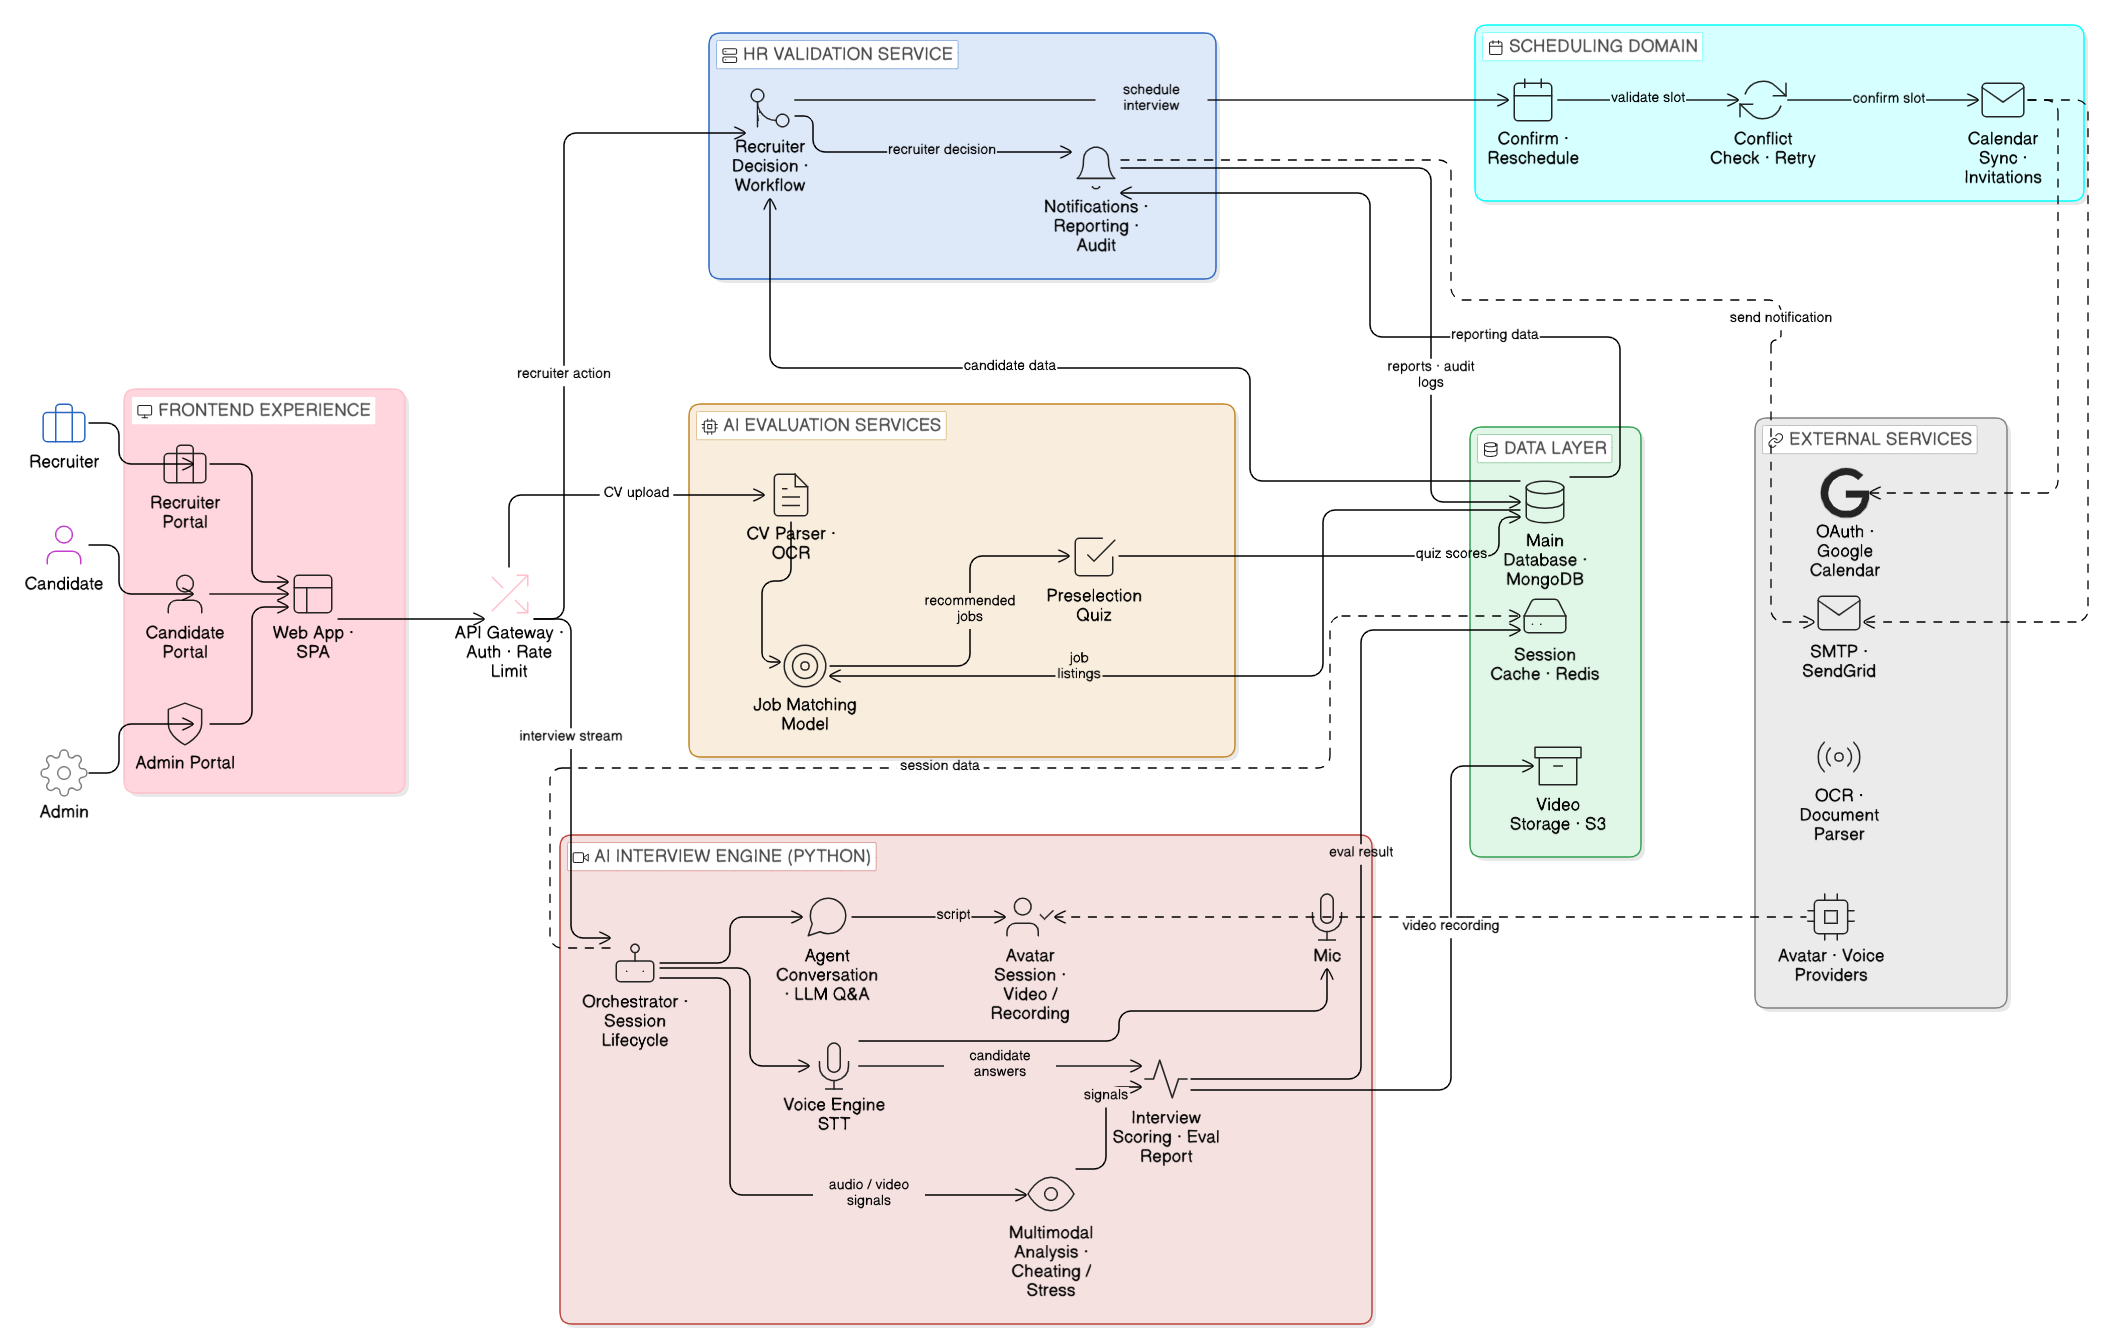
\includegraphics[width=0.95\textwidth]{../diagrams/diagram-export-4-11-2026-1_27_32-AM.png}
  \caption{Architecture globale de NextHire.}
  \label{fig:archi-globale}
\end{figure}

\subsection{Composants du système}

\subsubsection{Services}

Le tableau~\ref{tab:services} récapitule les services qui constituent la plateforme NextHire, leurs principales capacités (ce que chaque service prend en entrée et produit en sortie) ainsi que les protocoles de communication sur lesquels ils reposent.

\begin{table}[H]
  \centering
  \footnotesize
  \setlength{\tabcolsep}{4pt}
  \renewcommand{\arraystretch}{1.35}
  \begin{tabularx}{\textwidth}{|>{\raggedright\arraybackslash}p{2.3cm}|>{\raggedright\arraybackslash}p{2.4cm}|>{\raggedright\arraybackslash}X|>{\raggedright\arraybackslash}p{2.2cm}|}
    \hline
    \textbf{Service} & \textbf{Technologie} & \textbf{Capacités (entrée $\rightarrow$ sortie)} & \textbf{Protocoles} \\
    \hline
    Backend (point d'entrée / BFF) & Node.js / Express + Socket.IO & Reçoit tous les appels REST et WebSocket du client et vérifie le JWT $\rightarrow$ trafic authentifié routé vers le bon service ; orchestre les services Python & REST, WebSocket, WebRTC, JWT \\
    \hline
    Front-end & React 19 / Vite & Actions candidat et recruteur (offres, candidatures, passage d'entretien, tableaux de bord) $\rightarrow$ interfaces et appels API & REST, WebSocket \\
    \hline
    Interview Agent & Python / FastAPI & CV, contexte du poste et réponses du candidat $\rightarrow$ questions adaptatives (IRT), évaluation par réponse et score final ; état de session conservé dans Redis & REST, WebSocket, Redis \\
    \hline
    Speech Stack & Python / FastAPI & Audio du candidat $\rightarrow$ transcription (STT) ; texte de l'agent $\rightarrow$ synthèse vocale (TTS) et analyse de sentiment & REST \\
    \hline
    Face Verification & Python / Flask & Image webcam + photo de profil $\rightarrow$ vérification d'identité (\textit{embedding} 512-d, distance cosinus) & REST \\
    \hline
    YOLO Vision & Python / FastAPI & Trames webcam (base64) $\rightarrow$ objets et personnes détectés (téléphone, livre, écran, nombre de personnes) pour l'intégrité & REST \\
    \hline
    Analyse de sentiment (voix \& visage) & Python (Speech Stack + Analysis) & Segments audio et trames vidéo $\rightarrow$ labels d'émotion et scores de stress vocal qui enrichissent l'évaluation & REST \\
    \hline
    Analysis Service & Python / FastAPI + LangGraph & Transcription et événements de vision $\rightarrow$ rapport post-entretien, classement des candidats et aide à la décision & REST, Redis (RQ) \\
    \hline
    Scheduling & Python / FastAPI & Demandes de planification $\rightarrow$ événements d'agenda et courriels de notification & REST, Google Calendar, SMTP \\
    \hline
    Services IA (classiques) & Python / Flask & CV, profils et offres $\rightarrow$ parsing de CV, recommandation d'offres, scoring, génération de quiz et clustering (résultats JSON) & REST \\
    \hline
  \end{tabularx}
  \caption{Capacités des services (entrée $\rightarrow$ sortie) et protocoles de communication.}
  \label{tab:services}
\end{table}

\subsubsection{Protocoles de communication}

La plateforme combine trois protocoles selon la nature de l'échange :

\begin{itemize}
  \item \textbf{HTTP/REST} : opérations CRUD (offres, candidatures, résultats). Le
        \textit{front-end} passe par un proxy Vite vers le port 3001 ; le backend Node relaie
        ensuite vers les services Python (par exemple le parsing de CV sur le port 5002).
  \item \textbf{WebSocket (Socket.IO, port 3001)} : échanges en temps réel --- messagerie
        recruteur/candidat, entretien avec l'agent IA, et \textit{streaming} vocal vers le
        \textit{worker} STT (Faster-Whisper).
  \item \textbf{WebRTC} : visioconférence pair-à-pair des salles d'appel. La signalisation
        passe via Socket.IO et le relais média est assuré par la bibliothèque \texttt{wrtc}.
\end{itemize}

\subsubsection{Stockage des données}

Le stockage repose sur trois couches :

\begin{itemize}
  \item \textbf{MongoDB} (base \texttt{ai\_recruiter}, port 27017) : persistance partagée,
        via Mongoose côté Node.js (15 modèles au total, dont 8 entités métier principales --- les modèles auxiliaires complètent ce total) et PyMongo côté Python. Le modèle documentaire
        s'adapte à la variété des structures (transcriptions, analyses, rapports).
  \item \textbf{Redis} (port 6379) : état des sessions de l'agent (avec repli en mémoire) et
        file de tâches RQ à trois priorités (\texttt{high}, \texttt{default}, \texttt{low})
        pour les rapports post-entretien.
  \item \textbf{Disque local} : fichiers binaires déposés via Multer --- CV, enregistrements
        audio et photos de profil. Aucun stockage objet distant (S3) dans la version actuelle.
\end{itemize}

\section{Spécification des besoins}

Cette section formalise les exigences de la plateforme NextHire selon deux dimensions complémentaires : les besoins fonctionnels, qui décrivent ce que le système doit permettre à chaque acteur d'accomplir, et les besoins non-fonctionnels, qui précisent les contraintes de qualité que le système doit respecter indépendamment des fonctionnalités.

\subsection{Besoins fonctionnels}

Les besoins fonctionnels sont organisés par acteur. Chaque exigence est identifiée par un code de la forme \textbf{BF-X-\textit{nn}}, où \textbf{X} désigne l'acteur (\textbf{C} = Candidat, \textbf{R} = Recruteur, \textbf{A} = Administrateur) et \textit{nn} le numéro séquentiel. La priorité est exprimée sur trois niveaux : \textbf{H} (Haute), \textbf{M} (Moyenne), \textbf{B} (Basse).

\bigskip
\noindent\textbf{Acteur : Candidat}

\begin{table}[H]
  \centering
  \footnotesize
  \renewcommand{\arraystretch}{1.3}
  \begin{tabularx}{\textwidth}{|p{1.5cm}|X|c|}
    \hline
    \textbf{ID} & \textbf{Description} & \textbf{Priorité} \\
    \hline
    BF-C-01 & S'inscrire sur la plateforme et compléter son profil (informations personnelles, téléversement du CV). & H \\
    \hline
    BF-C-02 & Relier son compte LinkedIn à son profil afin d'importer automatiquement les données professionnelles. & M \\
    \hline
    BF-C-03 & Consulter les offres d'emploi disponibles et soumettre une candidature. & H \\
    \hline
    BF-C-04 & Recevoir des recommandations d'offres personnalisées fondées sur le profil et les compétences détectés dans le CV. & H \\
    \hline
    BF-C-05 & Passer un quiz de présélection associé à une offre avant d'accéder à l'entretien. & H \\
    \hline
    BF-C-06 & Planifier un entretien via le module de planification (\textit{scheduling}) intégré au calendrier. & H \\
    \hline
    BF-C-07 & Effectuer une vérification d'identité faciale avant le début de l'entretien. & H \\
    \hline
    BF-C-08 & Participer à un entretien en direct avec l'agent IA (avatar 3D parlant) au sein d'une salle d'appel sécurisée. & H \\
    \hline
    BF-C-09 & Consulter son score, la transcription et le rapport post-entretien généré par l'IA. & H \\
    \hline
    BF-C-10 & Échanger avec le recruteur via la messagerie en temps réel intégrée à la plateforme. & M \\
    \hline
    BF-C-11 & Recevoir des notifications par courriel sur l'évolution du statut de sa candidature. & M \\
    \hline
  \end{tabularx}
  \caption{Besoins fonctionnels -- acteur Candidat.}
  \label{tab:bf-candidat}
\end{table}

\bigskip
\noindent\textbf{Acteur : Recruteur}

\begin{table}[H]
  \centering
  \footnotesize
  \renewcommand{\arraystretch}{1.3}
  \begin{tabularx}{\textwidth}{|p{1.5cm}|X|c|}
    \hline
    \textbf{ID} & \textbf{Description} & \textbf{Priorité} \\
    \hline
    BF-R-01 & Créer et publier des offres d'emploi via l'assistant de création (\textit{Job Wizard}) guidé par l'IA. & H \\
    \hline
    BF-R-02 & Associer un quiz de présélection personnalisé à une offre (extension de la publication). & H \\
    \hline
    BF-R-03 & Consulter la liste des candidatures reçues ainsi que les profils détaillés des candidats. & H \\
    \hline
    BF-R-04 & Gérer et rejoindre les salles d'entretien en cours depuis le tableau de bord. & H \\
    \hline
    BF-R-05 & Consulter les résumés exécutifs, transcriptions complètes et scores pondérés générés automatiquement par l'IA. & H \\
    \hline
    BF-R-06 & Comparer et classer les candidats pour un poste donné à partir du moteur de ranking multicritères. & H \\
    \hline
    BF-R-07 & Consulter les rapports d'intégrité (niveau de risque, événements de fraude, captures d'écran d'anomalies). & H \\
    \hline
    BF-R-08 & Enregistrer une décision finale (acceptation ou refus) et déclencher la notification automatique du candidat. & H \\
    \hline
    BF-R-09 & Suivre les indicateurs de recrutement agrégés (taux de conversion, temps moyen, scores moyens) via le tableau de bord. & M \\
    \hline
  \end{tabularx}
  \caption{Besoins fonctionnels -- acteur Recruteur.}
  \label{tab:bf-recruteur}
\end{table}

\bigskip
\noindent\textbf{Acteur : Administrateur}

\begin{table}[H]
  \centering
  \footnotesize
  \renewcommand{\arraystretch}{1.3}
  \begin{tabularx}{\textwidth}{|p{1.5cm}|X|c|}
    \hline
    \textbf{ID} & \textbf{Description} & \textbf{Priorité} \\
    \hline
    BF-A-01 & Accéder au tableau de bord d'administration et consulter les statistiques globales de la plateforme. & H \\
    \hline
    BF-A-02 & Superviser l'ensemble des entités du système : utilisateurs, entreprises, offres, candidatures et entretiens. & H \\
    \hline
  \end{tabularx}
  \caption{Besoins fonctionnels -- acteur Administrateur.}
  \label{tab:bf-admin}
\end{table}

\subsection{Besoins non-fonctionnels}

Les besoins non-fonctionnels précisent les contraintes de qualité auxquelles la plateforme doit se conformer, indépendamment des fonctionnalités. Ils sont regroupés en sept catégories dans le tableau~\ref{tab:bnf}.

\begin{table}[H]
  \centering
  \footnotesize
  \renewcommand{\arraystretch}{1.45}
  \begin{tabularx}{\textwidth}{|>{\raggedright\arraybackslash}p{2.4cm}|>{\raggedright\arraybackslash}X|>{\raggedright\arraybackslash}X|}
    \hline
    \textbf{Catégorie} & \textbf{Exigence} & \textbf{Justification} \\
    \hline
    Performance & Délai inter-tour inférieur à 2\,s en déploiement GPU ; médiane mesurée de 807\,ms pour l'inférence LLM et de 937\,ms pour la synthèse vocale TTS. &
    Fluidité conversationnelle perçue : un délai supérieur à 2\,s rompt la continuité de l'échange et dégrade l'expérience candidat. \\
    \hline
    Sécurité & Authentification par jetons JWT (durée de validité 24\,h) ; contrôle d'accès RBAC à trois niveaux (Candidat, Recruteur, Administrateur) ; hachage des mots de passe par bcrypt ; comportement \textit{fail-closed} sur tout service IA indisponible. &
    Conformité aux recommandations OWASP ; protection contre les accès non autorisés et l'escalade de privilèges. \\
    \hline
    Scalabilité & Architecture micro-services indépendants ; état de session externalisé dans Redis ; montée en charge horizontale possible service par service. &
    Capacité à absorber des pics de demande sans refonte architecturale ; isolation des pannes entre services. \\
    \hline
    Confidentialité (RGPD) & Aucune image brute ne quitte le poste du candidat : seuls les vecteurs d'embedding (512 dimensions) sont transmis ; toutes les communications sont chiffrées en transit (HTTPS/TLS). &
    Conformité au Règlement Général sur la Protection des Données ; minimisation de la collecte et de l'exposition des données biométriques. \\
    \hline
    Disponibilité & Repli automatique en mémoire si Redis est indisponible ; redémarrage automatique des conteneurs via Docker Compose ; gestion \textit{fail-safe} dans les pipelines IA. &
    Continuité de service pendant un entretien en cours ; aucune interruption brutale pour le candidat. \\
    \hline
    Portabilité & Ensemble des services empaquetés dans des conteneurs Docker ; configuration centralisée par variables d'environnement (fichiers \texttt{.env}). &
    Déploiement reproductible sur tout hôte Linux ou Windows disposant de Docker, sans dépendance à l'environnement local. \\
    \hline
    Accessibilité & Interface web SPA (React\,19 / Vite) accessible depuis n'importe quel navigateur moderne sans installation côté candidat. &
    Élimination des frictions liées au téléchargement d'une application native ; compatibilité avec les contextes de recrutement à distance. \\
    \hline
  \end{tabularx}
  \caption{Besoins non-fonctionnels de la plateforme NextHire.}
  \label{tab:bnf}
\end{table}

\section{Diagrammes UML}

Cette section présente la modélisation du système à l'aide du langage UML : le diagramme de cas d'utilisation, le diagramme de classes et les diagrammes de séquence.

\subsection{Diagramme de cas d'utilisation}

La plateforme NextHire fait intervenir trois types d'acteurs : le \textbf{Candidat}, le \textbf{Recruteur} et l'\textbf{Administrateur}. L'authentification (inscription, connexion classique ou via Google OAuth) est un prérequis commun à tous les acteurs. L'IA n'est pas modélisée comme un acteur : ses interventions (agent d'entretien, analyse multimodale, scoring) sont des cas d'utilisation internes, inclus dans les processus du recruteur et du candidat. L'ajout d'un quiz de présélection à une offre est, quant à lui, modélisé comme une extension de la publication d'offre.

Les cas d’utilisation se répartissent entre les trois acteurs de la manière suivante.

\noindent\textbf{Candidat}

\begin{itemize}
  \item S’inscrire et compléter son profil (informations personnelles, téléversement du CV)
  \item Relier son compte LinkedIn à son profil
  \item Consulter les offres d’emploi et postuler
  \item Recevoir des recommandations d’offres basées sur son profil et ses compétences
  \item Passer un quiz de présélection associé à une offre
  \item Planifier un entretien via le module de planification (\textit{scheduling})
  \item Effectuer une vérification d’identité faciale avant l’entretien
  \item Participer à un entretien en direct avec l’agent IA dans une salle d’appel
  \item Consulter son score et son rapport post-entretien
  \item Échanger avec le recruteur via la messagerie en temps réel
  \item Recevoir des notifications par courriel sur le statut de sa candidature
\end{itemize}

\noindent\textbf{Recruteur}

\begin{itemize}
  \item Créer et publier des offres d’emploi via l’assistant de création (\textit{Job Wizard})
  \item Associer un quiz de présélection à une offre (extension de publication)
  \item Consulter les candidatures et les profils des candidats
  \item Gérer et rejoindre les salles d’entretien en cours
  \item Consulter les résumés, transcriptions et scores générés par l’IA
  \item Comparer et classer les candidats pour un poste donné
  \item Consulter les rapports d’intégrité (fraude, détection d’objets, changement de fenêtre)
  \item Prendre une décision finale (acceptation ou refus) et notifier le candidat
  \item Suivre les indicateurs de recrutement via le tableau de bord
\end{itemize}

\noindent\textbf{Administrateur}

\begin{itemize}
  \item Accéder au tableau de bord d’administration et aux statistiques globales
  \item Superviser les utilisateurs, entreprises, offres, candidatures et entretiens
\end{itemize}

La figure~\ref{fig:usecase} illustre l’ensemble de ces cas d’utilisation.

\begin{figure}[H]
  \centering
  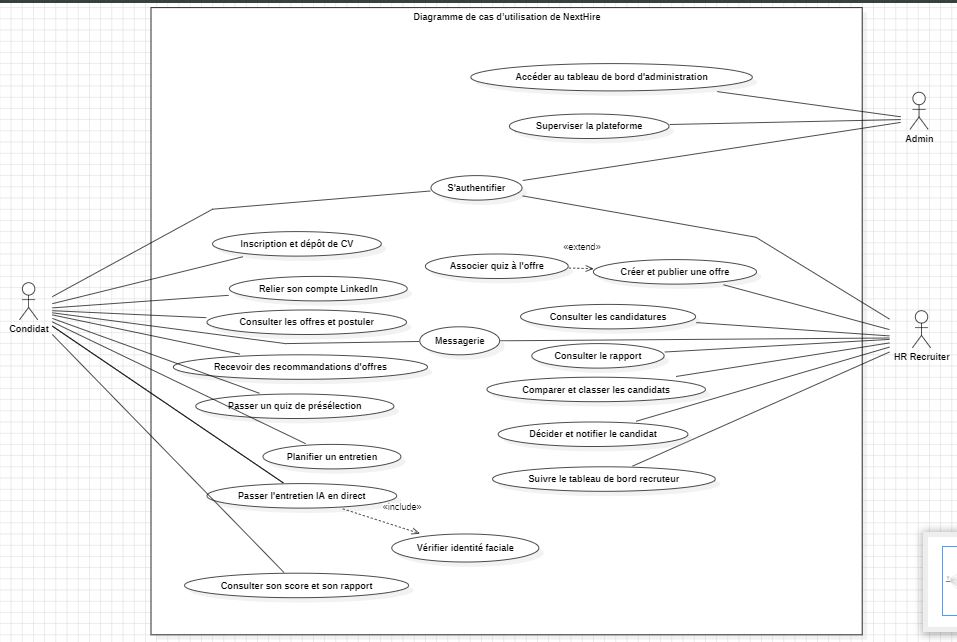
\includegraphics[width=\textwidth,keepaspectratio]{diagrams/usecase.JPG}
  \caption{Diagramme de cas d’utilisation de NextHire.}
  \label{fig:usecase}
\end{figure}

\subsection{Diagramme de classes}

Le diagramme de la figure~\ref{fig:classdiag} présente les principales entités du domaine
métier de NextHire, leurs attributs essentiels et les associations qui les relient. Ces
classes correspondent directement aux schémas Mongoose de la base de données
MongoDB \texttt{ai\_recruiter}.

Les entités principales sont :

\begin{itemize}
  \item \textbf{User} : entité centrale unique pour les trois rôles (ADMIN, ENTERPRISE,
        CANDIDATE). Elle porte le profil candidat, les informations de l'entreprise, la
        vérification faciale et les notifications.
  \item \textbf{Job} : offre d'emploi publiée par un recruteur, configurée via le Job Wizard
        (style d'entretien, critères d'évaluation pondérés, type d'entretien IA).
  \item \textbf{Application} : lien entre un candidat et une offre. Elle enregistre le score
        du quiz de présélection, le statut de la décision recruteur et le planning de
        l'entretien.
  \item \textbf{Quiz} : questionnaire de présélection généré par l'IA et associé à une offre
        d'emploi.
  \item \textbf{JobInterviewRoom} : salle partageable créée par le recruteur pour un poste.
        Chaque candidat y génère une session \textit{CallRoom} individuelle.
  \item \textbf{CallRoom} : session d'entretien IA individuelle. Elle contient la transcription,
        la vérification d'identité faciale, les événements d'intégrité (détection d'objets,
        changement de fenêtre) et le rapport final du recruteur.
  \item \textbf{ComparisonReport} : rapport de comparaison et de classement des candidats pour
        un poste, généré par l'agent IA d'analyse.
  \item \textbf{Message} : message échangé en temps réel entre un candidat et un recruteur
        via la messagerie intégrée.
\end{itemize}

\begin{figure}[H]
  \centering
  \resizebox{\textwidth}{!}{%
  \begin{tikzpicture}[
    font=\scriptsize,
    >={Stealth[length=2mm]},
  ]
  \tikzset{
    hdr/.style={draw, rectangle, fill=blue!12, minimum width=4.6cm, minimum height=0.65cm,
                align=center, font=\scriptsize\bfseries},
    atr/.style={draw, rectangle, fill=white, minimum width=4.6cm,
                align=left, text width=4.4cm, inner sep=3pt},
  }

  %% ─── USER ────────────────────────────────────────────────────────────────
  \node[hdr] (UH) at (0, 0) {User};
  \node[atr, anchor=north] (UA) at (UH.south) {
    +id : ObjectId\\
    +email : String\\
    +name : String\\
    +role : ADMIN $|$ ENTERPRISE $|$ CANDIDATE\\
    +isActive : Boolean\\
    +createdDate : Date
  };

  %% ─── JOB ─────────────────────────────────────────────────────────────────
  \node[hdr] (JH) at (7.5, 0) {Job};
  \node[atr, anchor=north] (JA) at (JH.south) {
    +id : ObjectId\\
    +title : String\\
    +status : DRAFT $|$ OPEN $|$ CLOSED\\
    +skills : [String]\\
    +interviewType : String\\
    +entrepriseId : ref User\\
    +createdAt : Date
  };

  %% ─── APPLICATION ─────────────────────────────────────────────────────────
  \node[hdr] (AH) at (0, -7) {Application};
  \node[atr, anchor=north] (AA) at (AH.south) {
    +id : ObjectId\\
    +candidateId : ref User\\
    +jobId : ref Job\\
    +status : PENDING $|$ INTERVIEW $|$ REJECTED\\
    +quizScore : Number\\
    +quizCompleted : Boolean\\
    +appliedAt : Date
  };

  %% ─── JOB INTERVIEW ROOM ──────────────────────────────────────────────────
  \node[hdr] (RH) at (7.5, -7) {JobInterviewRoom};
  \node[atr, anchor=north] (RA) at (RH.south) {
    +id : ObjectId\\
    +job : ref Job\\
    +company : ref User\\
    +slug : String\\
    +status : open $|$ closed\\
    +totalSessions : Number
  };

  %% ─── CALL ROOM ───────────────────────────────────────────────────────────
  \node[hdr] (CH) at (0, -14) {CallRoom};
  \node[atr, anchor=north] (CA) at (CH.south) {
    +id : ObjectId\\
    +roomId : String\\
    +initiator : ref User\\
    +candidate : ref User\\
    +job : ref Job\\
    +status : waiting $|$ active $|$ ended\\
    +transcription : Object\\
    +faceVerification : Object\\
    +integrityReport : Object\\
    +recruiterReport : Object
  };

  %% ─── COMPARISON REPORT ───────────────────────────────────────────────────
  \node[hdr] (CRH) at (7.5, -14) {ComparisonReport};
  \node[atr, anchor=north] (CRA) at (CRH.south) {
    +id : ObjectId\\
    +job : ref Job\\
    +company : ref User\\
    +rankings : [CandidateRanking]\\
    +status : pending $|$ ready $|$ failed\\
    +executiveSummary : String\\
    +generatedAt : Date
  };

  %% ─── QUIZ ────────────────────────────────────────────────────────────────
  \node[hdr] (QH) at (14, -3) {Quiz};
  \node[atr, anchor=north] (QA) at (QH.south) {
    +id : ObjectId\\
    +jobId : ref Job\\
    +questions[].type : QCM $|$ vrai-faux\\
    +questions[].options : [String]\\
    +questions[].correctAnswer : Number\\
    +questions[].difficulty : String
  };

  %% ─── MESSAGE ─────────────────────────────────────────────────────────────
  \node[hdr] (MH) at (-6.5, -7) {Message};
  \node[atr, anchor=north] (MA) at (MH.south) {
    +id : ObjectId\\
    +from : ref User\\
    +to : ref User\\
    +text : String\\
    +timestamp : Date\\
    +read : Boolean
  };

  %% ─── RELATIONSHIPS ───────────────────────────────────────────────────────

  % User --[1 posts 0..*]--> Job
  \draw[->] (UH.east) --
    node[above, font=\tiny] {1 \quad posts \quad 0..*}
    (JH.west);

  % User --[0..*]--> Application  (candidate applies)
  \draw[->] (UA.south) --
    node[right, font=\tiny] {0..* applies}
    (AH.north);

  % Job --[0..*]--> Application  (job receives)
  \draw[->] (JA.south west) --
    node[below right, font=\tiny] {0..*}
    (AH.north east);

  % Job --[0..1]--> Quiz
  \draw[->] (JH.east) -|
    node[above, font=\tiny, pos=0.25] {has \quad 0..1}
    (QH.north);

  % Job --[0..1]--> JobInterviewRoom
  \draw[->] (JA.south) --
    node[right, font=\tiny] {0..1}
    (RH.north);

  % JobInterviewRoom --[0..*]--> CallRoom
  \draw[->] (RA.south west) --
    node[below left, font=\tiny] {0..*}
    (CH.north east);

  % JobInterviewRoom --[0..1]--> ComparisonReport
  \draw[->] (RA.south) --
    node[right, font=\tiny] {0..1}
    (CRH.north);

  % User <--> Message  (from / to)
  \draw[->] (UA.west) -- ++(-0.4,0) |-
    node[left, font=\tiny, pos=0.7] {from/to}
    (MH.north);

  % ComparisonReport --[for]--> Job  (dashed reference)
  \draw[->, dashed] (CRH.east) -- ++(0.4,0) |-
    node[right, font=\tiny, pos=0.25] {for}
    (JA.east);

  \end{tikzpicture}%
  }
  \caption{Diagramme de classes des entités principales de NextHire (base \texttt{ai\_recruiter}).}
  \label{fig:classdiag}
\end{figure}

\subsection{Diagrammes de séquence}

\subsubsection{Session d'entretien IA}

La figure~\ref{fig:seq-interview} illustre le flux de messages d'une session d'entretien IA NextHire, de l'initialisation de la salle jusqu'à la génération du rapport final.

Les étapes clés sont les suivantes.

\begin{sloppypar}
\begin{enumerate}
  \item \textbf{Initialisation.} Le candidat ouvre la page d'entretien. Le client React envoie
        une requête \texttt{GET} vers \texttt{/api/callrooms/\{roomId\}} au backend Node.js,
        qui récupère le document \texttt{CallRoom} dans MongoDB (contexte du poste, profil
        candidat, statut de la session) et retourne ces données au client.

  \item \textbf{Vérification d'identité.} Le candidat soumet une image de sa webcam pour
        la vérification faciale. Le backend appelle le service Face Verify (Python, port 8011),
        qui compare l'embedding de l'image en direct avec celui enregistré lors de l'inscription
        (similarité cosinus, modèle InsightFace \textit{buffalo-l}) et autorise l'entretien
        si le seuil de correspondance est atteint.

  \item \textbf{Démarrage de l'entretien.} Le client établit une connexion Socket.IO avec le
        backend. Celui-ci initialise une session auprès de l'Interview Agent via REST. L'agent
        crée un objet \texttt{InterviewState} en mémoire, appelle le LLM Groq avec le prompt
        système pour générer la question d'ouverture, transmet le texte à Edge TTS pour la
        synthèse vocale, et diffuse l'audio au candidat.

  \item \textbf{Boucle Q\&A.} Le candidat répond oralement. L'audio PCM est envoyé au backend
        via Socket.IO, transcrit par Faster Whisper (STT), puis transmis à l'Interview Agent.
        L'agent évalue la réponse via le LLM (scoring IRT-lite, mise à jour du score de
        capacité adaptative) et génère la question suivante. La boucle se répète jusqu'à ce
        que le champ \texttt{done} retourné par le LLM soit \texttt{true}.

  \item \textbf{Fin de l'entretien.} L'agent retourne l'évaluation finale avec la transcription
        complète. Le backend construit le rapport recruteur, le persiste dans MongoDB, déclenche
        l'analyse post-entretien en arrière-plan (service Analysis), et notifie le client via
        Socket.IO.
\end{enumerate}
\end{sloppypar}

\begin{figure}[H]
  \centering
  \resizebox{\textwidth}{!}{%
  \begin{tikzpicture}[
    font=\scriptsize,
    >={Stealth[length=2mm]},
    msg/.style={->, thin},
    ret/.style={->, thin, dashed},
    lbl/.style={font=\tiny, fill=white, inner sep=1pt, midway, above},
    lifeline/.style={dashed, thin, gray!70},
    phdr/.style={draw, fill=blue!12, rounded corners=2pt, align=center,
                 font=\scriptsize\bfseries, minimum height=0.65cm, minimum width=2.8cm},
  ]

  %% ── Participant boxes ──────────────────────────────────────────────────
  \node[phdr] at ( 0, 0) {React\\(Client)};
  \node[phdr] at ( 4, 0) {Node.js\\(:3001)};
  \node[phdr] at ( 8, 0) {Interview Agent\\(:8013)};
  \node[phdr] at (12, 0) {Faster Whisper\\(STT :8012)};
  \node[phdr] at (16, 0) {Groq\\(LLM API)};
  \node[phdr] at (20, 0) {Edge TTS\\(:8003)};
  \node[phdr] at (24, 0) {MongoDB};

  %% ── Lifelines ──────────────────────────────────────────────────────────
  \draw[lifeline] ( 0,-0.38) -- ( 0,-21.5);
  \draw[lifeline] ( 4,-0.38) -- ( 4,-21.5);
  \draw[lifeline] ( 8,-0.38) -- ( 8,-21.5);
  \draw[lifeline] (12,-0.38) -- (12,-21.5);
  \draw[lifeline] (16,-0.38) -- (16,-21.5);
  \draw[lifeline] (20,-0.38) -- (20,-21.5);
  \draw[lifeline] (24,-0.38) -- (24,-21.5);

  %% ════════════════════════════════════════════════════════════════════════
  %% 1. Initialisation
  %% ════════════════════════════════════════════════════════════════════════
  \node[font=\tiny\bfseries, anchor=east] at (-0.3,-0.75) {1.};
  \draw[msg] ( 0,-0.75) -- node[lbl] {GET /api/callrooms/:roomId} (4,-0.75);
  \draw[msg] ( 4,-1.30) -- node[lbl] {findOne(roomId)} (24,-1.30);
  \draw[ret] (24,-1.85) -- node[lbl] {CallRoom \{jobContext, status, candidateInfo\}} (4,-1.85);
  \draw[ret] ( 4,-2.40) -- node[lbl] {200 OK \{roomId, jobContext\}} (0,-2.40);

  %% ════════════════════════════════════════════════════════════════════════
  %% 2. Vérification d'identité faciale
  %% ════════════════════════════════════════════════════════════════════════
  \node[font=\tiny\bfseries, anchor=east] at (-0.3,-2.85) {2.};
  \draw[msg] (0,-2.85) -- node[lbl] {POST /face-verify \{webcam\_frame\}} (4,-2.85);
  \draw[draw=orange!70, fill=orange!8, rounded corners=1pt, thin]
    (4.1,-3.10) rectangle (7.9,-3.65);
  \node[font=\tiny, anchor=west] at (4.2,-3.38)
    {[Face Verify :8011] compare\_embedding};
  \draw[ret] (4,-3.95) -- node[lbl] {\{allowInterview: true, similarity: 0.92\}} (0,-3.95);
  \draw[msg] (4,-4.45) -- node[lbl] {PATCH callrooms \{faceVerification: matched\}} (24,-4.45);

  %% ════════════════════════════════════════════════════════════════════════
  %% 3. Démarrage de l'entretien
  %% ════════════════════════════════════════════════════════════════════════
  \node[font=\tiny\bfseries, anchor=east] at (-0.3,-4.95) {3.};
  \draw[msg] (0,-4.95) -- node[lbl] {Socket.IO connect(roomId)} (4,-4.95);
  \draw[msg] (4,-5.55) -- node[lbl] {POST /init-session \{jobContext, candidateProfile, style\}} (8,-5.55);
  %% self-arrow: create InterviewState
  \draw[->] (8,-6.15) -- ++(0.6,0) -- ++(0,-0.40) -- ++(-0.6,0);
  \node[font=\tiny, anchor=west] at (8.70,-6.35) {create InterviewState};
  \draw[msg] (8,-6.90) -- node[lbl] {chat.completions(COMPACT\_SYSTEM + opening\_prompt)} (16,-6.90);
  \draw[ret] (16,-7.50) -- node[lbl] {\{next\_question, score:0.5, done:false\}} (8,-7.50);
  \draw[ret] ( 8,-8.05) -- node[lbl] {\{question\_text\}} (4,-8.05);
  \draw[msg] ( 4,-8.55) -- node[lbl] {synthesize(question\_text)} (20,-8.55);
  \draw[ret] (20,-9.10) -- node[lbl] {audio stream} (4,-9.10);
  \draw[ret] ( 4,-9.60) -- node[lbl] {emit("agent-audio",\ audio)} (0,-9.60);

  %% ════════════════════════════════════════════════════════════════════════
  %% 4. Boucle Q&A
  %% ════════════════════════════════════════════════════════════════════════
  \node[font=\tiny\bfseries, anchor=east] at (-0.3,-10.1) {4.};
  %% Loop frame
  \draw[draw=green!50!black, fill=green!5, rounded corners=3pt, dashed, thin]
    (-0.3,-10.1) rectangle (21.3,-18.5);
  \node[font=\tiny\bfseries, text=green!40!black, anchor=north west]
    at (-0.2,-10.15) {loop [répéter jusqu'à done = true]};

  \draw[msg] ( 0,-10.75) -- node[lbl] {emit("audio-chunk",\ PCM\_audio)} (4,-10.75);
  \draw[msg] ( 4,-11.35) -- node[lbl] {POST /transcribe \{audio\}} (12,-11.35);
  \draw[ret] (12,-11.95) -- node[lbl] {\{text: transcript\}} (4,-11.95);
  \draw[msg] ( 4,-12.55) -- node[lbl] {POST /next-turn \{interview\_id, transcript\}} (8,-12.55);
  %% self-arrow: IRT update
  \draw[->] (8,-13.15) -- ++(0.6,0) -- ++(0,-0.40) -- ++(-0.6,0);
  \node[font=\tiny, anchor=west] at (8.70,-13.35)
    {update\_theta(score,\ confidence) --- IRT-lite};
  \draw[msg] ( 8,-13.95) -- node[lbl] {chat.completions(contexte + réponse candidat)} (16,-13.95);
  \draw[ret] (16,-14.55) -- node[lbl] {\{score, next\_question, difficulty, done\}} (8,-14.55);
  \draw[ret] ( 8,-15.15) -- node[lbl] {\{question, score, done\}} (4,-15.15);
  \draw[msg] ( 4,-15.75) -- node[lbl] {synthesize(next\_question) [if !done]} (20,-15.75);
  \draw[ret] (20,-16.35) -- node[lbl] {audio stream} (4,-16.35);
  \draw[ret] ( 4,-16.95) -- node[lbl] {emit("agent-audio",\ audio)} (0,-16.95);
  %% guard box
  \draw[draw=gray!50, fill=gray!8, rounded corners=1pt, thin]
    (0.5,-17.75) rectangle (7.5,-18.25);
  \node[font=\tiny] at (4.0,-18.00)
    {[done = true] $\Rightarrow$ sortie de boucle};

  %% ════════════════════════════════════════════════════════════════════════
  %% 5. Fin de l'entretien
  %% ════════════════════════════════════════════════════════════════════════
  \node[font=\tiny\bfseries, anchor=east] at (-0.3,-18.8) {5.};
  \draw[ret] ( 8,-18.80) -- node[lbl] {\{done:true, final\_evaluation, transcript\}} (4,-18.80);
  \draw[msg] ( 4,-19.40) -- node[lbl] {PATCH /callrooms/:id \{status:ended, recruiterReport\}} (24,-19.40);
  \draw[ret] (24,-19.95) -- node[lbl] {200 OK} (4,-19.95);
  \draw[msg] ( 4,-20.50) -- node[lbl] {POST /analyze-video (async, fire-and-forget)} (8,-20.50);
  \draw[ret] ( 4,-21.05) -- node[lbl] {emit("interview-ended",\ \{score, summary\})} (0,-21.05);

  \end{tikzpicture}%
  }
  \caption{Diagramme de séquence --- session d'entretien IA NextHire.}
  \label{fig:seq-interview}
\end{figure}

% ─────────────────────────────────────────────────────────────────────────────
\subsubsection{Surveillance d'intégrité en temps réel}

La figure~\ref{fig:seq-integrity} illustre le flux de surveillance d'intégrité qui s'exécute
en parallèle de chaque session d'entretien. Le système combine la détection d'objets (YOLO),
la vérification continue d'identité (Face Verify) et la surveillance des actions navigateur
pour détecter en temps réel tout comportement suspect.

\begin{sloppypar}
\begin{enumerate}
  \item \textbf{Activation.} À l'ouverture de la salle d'entretien, le backend vérifie que
        le profil facial du candidat est bien enregistré (embedding InsightFace) et notifie
        le client que la surveillance est active.

  \item \textbf{Boucle d'analyse vidéo.} Durant l'entretien, le client envoie des trames
        vidéo encodées en Base64 via Socket.IO. Le backend les transmet en parallèle au service
        YOLO Vision (détection de téléphone, document, écran, personnes multiples) et au
        service Face Verify (correspondance d'identité par similarité cosinus). En cas de
        violation détectée, l'événement est enregistré dans le document \texttt{CallRoom}
        avec son type, sa sévérité et l'identifiant de la question en cours.

  \item \textbf{Événements navigateur.} La page surveille les changements d'onglet, la
        sortie du plein écran et les tentatives de copier-coller, et les transmet immédiatement
        au backend. Ces événements sont enregistrés avec la sévérité \textit{critical}.

  \item \textbf{Rapport d'intégrité.} À la fin de la session, le backend agrège tous les
        événements, calcule un score de risque global et persiste le
        \texttt{integrityReport} (niveau de risque, synthèse, recommandation recruteur)
        dans MongoDB.
\end{enumerate}
\end{sloppypar}

\begin{figure}[H]
  \centering
  \resizebox{\textwidth}{!}{%
  \begin{tikzpicture}[
    font=\scriptsize,
    >={Stealth[length=2mm]},
    msg/.style={->, thin},
    ret/.style={->, thin, dashed},
    lbl/.style={font=\tiny, fill=white, inner sep=1pt, midway, above},
    lifeline/.style={dashed, thin, gray!70},
    phdr/.style={draw, fill=blue!12, rounded corners=2pt, align=center,
                 font=\scriptsize\bfseries, minimum height=0.65cm, minimum width=2.7cm},
  ]

  %% ── Participants ──────────────────────────────────────────────────────
  \node[phdr] at ( 0, 0) {React\\(Client)};
  \node[phdr] at ( 4, 0) {Node.js\\(:3001)};
  \node[phdr] at ( 9, 0) {YOLO Vision\\(:8001)};
  \node[phdr] at (14, 0) {Face Verify\\(:8011)};
  \node[phdr] at (19, 0) {MongoDB};

  %% ── Lifelines ─────────────────────────────────────────────────────────
  \draw[lifeline] ( 0,-0.38) -- ( 0,-15.0);
  \draw[lifeline] ( 4,-0.38) -- ( 4,-15.0);
  \draw[lifeline] ( 9,-0.38) -- ( 9,-15.0);
  \draw[lifeline] (14,-0.38) -- (14,-15.0);
  \draw[lifeline] (19,-0.38) -- (19,-15.0);

  %% ════════════════════════════════════════════════════════════════════════
  %% 1. Activation
  %% ════════════════════════════════════════════════════════════════════════
  \node[font=\tiny\bfseries, anchor=east] at (-0.3,-0.75) {1.};
  \draw[msg] ( 0,-0.75) -- node[lbl] {Socket.IO connect(roomId) + startMonitoring} (4,-0.75);
  \draw[msg] ( 4,-1.40) -- node[lbl] {GET /enrollment-status \{candidateId\}} (14,-1.40);
  \draw[ret] (14,-1.95) -- node[lbl] {\{enrolled: true, threshold: 0.55\}} (4,-1.95);
  \draw[ret] ( 4,-2.50) -- node[lbl] {emit("monitoring-ready")} (0,-2.50);

  %% ════════════════════════════════════════════════════════════════════════
  %% 2. Loop — analyse vidéo
  %% ════════════════════════════════════════════════════════════════════════
  \node[font=\tiny\bfseries, anchor=east] at (-0.3,-2.95) {2.};
  \draw[draw=green!50!black, fill=green!5, rounded corners=3pt, dashed, thin]
    (-0.3,-2.95) rectangle (20.3,-9.70);
  \node[font=\tiny\bfseries, text=green!40!black, anchor=north west]
    at (-0.2,-3.00) {loop [chaque trame vidéo --- 1 img/s]};

  \draw[msg] ( 0,-3.65) -- node[lbl] {emit("video-frame", \{frame: base64, questionId\})} (4,-3.65);
  \draw[msg] ( 4,-4.25) -- node[lbl] {POST /detect \{frame\}} (9,-4.25);
  \draw[ret] ( 9,-4.85) -- node[lbl] {\{objects: [...], persons: N\}} (4,-4.85);
  \draw[msg] ( 4,-5.45) -- node[lbl] {POST /verify \{frame\}} (14,-5.45);
  \draw[ret] (14,-6.05) -- node[lbl] {\{status, similarity\}} (4,-6.05);

  %% alt: violation détectée
  \draw[draw=red!50, fill=red!4, rounded corners=2pt, thin]
    (0.4,-6.55) rectangle (19.7,-9.30);
  \node[font=\tiny\bfseries, text=red!60!black, anchor=north west]
    at (0.5,-6.60) {alt [violation détectée — PHONE\_VISIBLE, MULTIPLE\_FACES, TAB\_SWITCH, ...]};
  \draw[msg] ( 4,-7.25) -- node[lbl] {enregistrer violation \{type, severity, evidence, questionId\}} (19,-7.25);
  \draw[ret] ( 4,-7.95) -- node[lbl] {emit("integrity-alert", \{type, severity\})} (0,-7.95);
  \draw[thin, gray!50] (0.4,-8.45) -- (19.7,-8.45);
  \node[font=\tiny, text=gray!55, anchor=west] at (0.5,-8.35) {else};
  \draw[ret] ( 4,-8.90) -- node[lbl] {emit("frame-ok")} (0,-8.90);

  %% ════════════════════════════════════════════════════════════════════════
  %% 3. Événements navigateur
  %% ════════════════════════════════════════════════════════════════════════
  \node[font=\tiny\bfseries, anchor=east] at (-0.3,-10.15) {3.};
  \draw[msg] ( 0,-10.15) -- node[lbl] {emit("browser-event", \{type: TAB\_SWITCH | FULLSCREEN\_EXIT\})} (4,-10.15);
  \draw[msg] ( 4,-10.80) -- node[lbl] {enregistrer événement \{type, severity: critical\}} (19,-10.80);
  \draw[ret] ( 4,-11.40) -- node[lbl] {emit("integrity-alert", \{type, severity: critical\})} (0,-11.40);

  %% ════════════════════════════════════════════════════════════════════════
  %% 4. Rapport d'intégrité
  %% ════════════════════════════════════════════════════════════════════════
  \node[font=\tiny\bfseries, anchor=east] at (-0.3,-12.00) {4.};
  \draw[->] (4,-12.00) -- ++(0.6,0) -- ++(0,-0.40) -- ++(-0.6,0);
  \node[font=\tiny, anchor=west] at (4.70,-12.20) {generateIntegrityReport(roomId)};
  \draw[msg] ( 4,-12.80) -- node[lbl] {sauvegarder integrityReport \{riskLevel, riskScore, keyFindings\}} (19,-12.80);
  \draw[ret] (19,-13.40) -- node[lbl] {200 OK} (4,-13.40);
  \draw[ret] ( 4,-13.90) -- node[lbl] {emit("integrity-report-ready", \{riskLevel, score\})} (0,-13.90);

  \end{tikzpicture}%
  }
  \caption{Diagramme de séquence --- surveillance d'intégrité en temps réel.}
  \label{fig:seq-integrity}
\end{figure}

% ─────────────────────────────────────────────────────────────────────────────
\subsubsection{Génération du rapport post-entretien}

La figure~\ref{fig:seq-report} illustre le flux de génération du rapport post-entretien,
déclenché automatiquement dès la fin de la session. Le rapport final combine l'évaluation
pondérée de l'agent IA (technique 40\,\%, communication 20\,\%, expérience 20\,\%,
comportement 10\,\%, intégrité 10\,\%) et l'analyse multimodale produite par le service
Analysis via un pipeline LangGraph.

\begin{sloppypar}
\begin{enumerate}
  \item \textbf{Déclenchement.} Dès que l'agent retourne \texttt{done:true}, le backend
        récupère le snapshot de la session (transcription, évaluations IRT, critères du
        poste) depuis MongoDB pour construire l'évaluation pondérée.

  \item \textbf{Analyse post-entretien.} Le backend déclenche le service Analysis en
        arrière-plan (fire-and-forget). Ce service exécute un pipeline LangGraph : il
        récupère le document complet de la session, appelle le LLM NVIDIA NIM (\\texttt{meta/llama-3.3-70b-instruct}) pour analyser
        la transcription, évaluer les compétences et produire des recommandations, puis
        persiste la timeline comportementale dans MongoDB.

  \item \textbf{Construction du rapport recruteur.} Le backend assemble le rapport final
        à partir du snapshot de l'agent, du rapport d'intégrité et des résultats de
        l'analyse, le persiste dans MongoDB et notifie le client de la fin de la session.

  \item \textbf{Consultation.} Le recruteur ouvre la fiche depuis le tableau de bord. Le
        backend renvoie le rapport complet (scores, violations, transcription,
        recommandations de l'IA).
\end{enumerate}
\end{sloppypar}

\begin{figure}[H]
  \centering
  \resizebox{\textwidth}{!}{%
  \begin{tikzpicture}[
    font=\scriptsize,
    >={Stealth[length=2mm]},
    msg/.style={->, thin},
    ret/.style={->, thin, dashed},
    lbl/.style={font=\tiny, fill=white, inner sep=1pt, midway, above},
    lifeline/.style={dashed, thin, gray!70},
    phdr/.style={draw, fill=blue!12, rounded corners=2pt, align=center,
                 font=\scriptsize\bfseries, minimum height=0.65cm, minimum width=2.7cm},
  ]

  %% ── Participants ──────────────────────────────────────────────────────
  \node[phdr] at ( 0,  0) {React\\(Recruteur)};
  \node[phdr] at ( 4.5,0) {Node.js\\(:3001)};
  \node[phdr] at (10,  0) {Analysis Service\\(:8090)};
  \node[phdr] at (15.5,0) {NVIDIA NIM\\(LLM API)};
  \node[phdr] at (21,  0) {MongoDB};

  %% ── Lifelines ─────────────────────────────────────────────────────────
  \draw[lifeline] ( 0,  -0.38) -- ( 0,  -14.5);
  \draw[lifeline] ( 4.5,-0.38) -- ( 4.5,-14.5);
  \draw[lifeline] (10,  -0.38) -- (10,  -14.5);
  \draw[lifeline] (15.5,-0.38) -- (15.5,-14.5);
  \draw[lifeline] (21,  -0.38) -- (21,  -14.5);

  %% ════════════════════════════════════════════════════════════════════════
  %% 1. Déclenchement
  %% ════════════════════════════════════════════════════════════════════════
  \node[font=\tiny\bfseries, anchor=east] at (-0.3,-0.75) {1.};
  \draw[->] (4.5,-0.75) -- ++(0.6,0) -- ++(0,-0.40) -- ++(-0.6,0);
  \node[font=\tiny, anchor=west] at (5.15,-0.95)
    {buildWeightedEvaluation(agentSnapshot, criteria)};
  \draw[msg] (4.5,-1.60) -- node[lbl] {findOne(callRoom) --- transcript + integrityEvents} (21,-1.60);
  \draw[ret] (21,-2.20) -- node[lbl] {\{transcription, evaluations, violations\}} (4.5,-2.20);

  %% ════════════════════════════════════════════════════════════════════════
  %% 2. Analyse post-entretien
  %% ════════════════════════════════════════════════════════════════════════
  \node[font=\tiny\bfseries, anchor=east] at (-0.3,-2.85) {2.};
  \draw[msg] (4.5,-2.85) -- node[lbl] {POST /api/interviews/\{id\}/analyze-video} (10,-2.85);
  \draw[msg] (10,  -3.50) -- node[lbl] {findOne(callRoom) \{full document\}} (21,-3.50);
  \draw[ret] (21,  -4.10) -- node[lbl] {\{transcription, visionEvents, agentEvaluations\}} (10,-4.10);
  %% self-arrow: LangGraph pipeline
  \draw[->] (10,-4.70) -- ++(0.6,0) -- ++(0,-0.40) -- ++(-0.6,0);
  \node[font=\tiny, anchor=west] at (10.70,-4.90) {LangGraph pipeline (analyse multimodale)};
  \draw[msg] (10,  -5.60) -- node[lbl] {chat.completions(transcript + job\_context + criteria)} (15.5,-5.60);
  \draw[ret] (15.5,-6.20) -- node[lbl] {\{skills\_scores, strengths, gaps, recommendations\}} (10,-6.20);
  \draw[msg] (10,  -6.85) -- node[lbl] {PATCH callRoom \{behavioralTimeline, analyzed: true\}} (21,-6.85);
  \draw[ret] (10,  -7.45) -- node[lbl] {\{status: done\}} (4.5,-7.45);

  %% ════════════════════════════════════════════════════════════════════════
  %% 3. Construction du rapport recruteur
  %% ════════════════════════════════════════════════════════════════════════
  \node[font=\tiny\bfseries, anchor=east] at (-0.3,-8.10) {3.};
  \draw[->] (4.5,-8.10) -- ++(0.6,0) -- ++(0,-0.40) -- ++(-0.6,0);
  \node[font=\tiny, anchor=west] at (5.15,-8.30)
    {buildRecruiterReport(snapshot, integrity, analysis)};
  \draw[msg] (4.5,-9.00) -- node[lbl] {PATCH callRoom \{status:ended, recruiterReport, integrityReport\}} (21,-9.00);
  \draw[ret] (21, -9.60) -- node[lbl] {200 OK} (4.5,-9.60);
  \draw[ret] (4.5,-10.15) -- node[lbl] {emit("interview-ended", \{overallScore, reportReady: true\})} (0,-10.15);

  %% ════════════════════════════════════════════════════════════════════════
  %% 4. Consultation du rapport (recruteur)
  %% ════════════════════════════════════════════════════════════════════════
  \node[font=\tiny\bfseries, anchor=east] at (-0.3,-10.90) {4.};
  \draw[msg] ( 0,-10.90) -- node[lbl] {GET /api/callrooms/\{id\}} (4.5,-10.90);
  \draw[msg] (4.5,-11.55) -- node[lbl] {findOne(callRoom).populate(job, user)} (21,-11.55);
  \draw[ret] (21, -12.15) -- node[lbl] {\{recruiterReport, integrityReport, transcript, score\}} (4.5,-12.15);
  %% scoring breakdown note
  \draw[draw=orange!60, fill=orange!6, rounded corners=1pt, thin]
    (4.6,-12.70) rectangle (12.5,-13.35);
  \node[font=\tiny, anchor=west] at (4.7,-13.02)
    {tech 40\% · comm 20\% · exp 20\% · behav 10\% · integrity 10\%};
  \draw[ret] (4.5,-13.80) -- node[lbl] {200 OK \{fullReport, violations, ranking\}} (0,-13.80);

  \end{tikzpicture}%
  }
  \caption{Diagramme de séquence --- génération du rapport post-entretien.}
  \label{fig:seq-report}
\end{figure}

\section{Schéma de la base de données}

\subsection{Diagramme entité-relation}

La figure~\ref{fig:erd} présente le diagramme entité-relation de la base de données MongoDB
\texttt{ai\_recruiter}. Chaque entité correspond à une collection Mongoose. Les références
entre documents sont représentées par des champs \texttt{ref} (équivalents MongoDB des clés
étrangères relationnelles).

\begin{figure}[H]
  \centering
  \resizebox{\textwidth}{!}{%
  \begin{tikzpicture}[
    font=\scriptsize,
    >={Stealth[length=1.5mm]},
  ]
  \tikzset{
    hdr/.style={draw, fill=blue!15, minimum width=4.0cm, minimum height=0.55cm,
                align=center, font=\tiny\bfseries},
    bdy/.style={draw, fill=white, minimum width=4.0cm, align=left,
                text width=3.8cm, inner sep=2.5pt, font=\tiny},
    rel/.style={thin},
    lbl/.style={font=\tiny, fill=white, inner sep=1pt},
  }

  %% ── USER ──────────────────────────────────────────────────────────────
  \node[hdr] (UH) at (7.5, 0) {User};
  \node[bdy, anchor=north] (UB) at (UH.south) {
    \textbf{PK}\ \_id : ObjectId\\
    email : String (unique)\\
    name : String\\
    role : ENUM (ADMIN, ENTERPRISE, CANDIDATE)\\
    isActive : Boolean\\
    createdDate : Date
  };

  %% ── MESSAGE ───────────────────────────────────────────────────────────
  \node[hdr] (MH) at (17, 0) {Message};
  \node[bdy, anchor=north] (MB) at (MH.south) {
    \textbf{PK}\ \_id : ObjectId\\
    \textbf{FK}\ from : ref User\\
    \textbf{FK}\ to : ref User\\
    text : String\\
    timestamp : Date\\
    read : Boolean
  };

  %% ── JOB ───────────────────────────────────────────────────────────────
  \node[hdr] (JH) at (0, -7) {Job};
  \node[bdy, anchor=north] (JB) at (JH.south) {
    \textbf{PK}\ \_id : ObjectId\\
    \textbf{FK}\ entrepriseId : ref User\\
    title : String\\
    status : ENUM (DRAFT, OPEN, CLOSED)\\
    skills : [String]\\
    interviewType : String\\
    createdAt : Date
  };

  %% ── APPLICATION ───────────────────────────────────────────────────────
  \node[hdr] (AH) at (7.5, -7) {Application};
  \node[bdy, anchor=north] (AB) at (AH.south) {
    \textbf{PK}\ \_id : ObjectId\\
    \textbf{FK}\ candidateId : ref User\\
    \textbf{FK}\ jobId : ref Job\\
    \textbf{FK}\ enterpriseId : ref User\\
    status : ENUM (PENDING, INTERVIEW, REJECTED)\\
    quizScore : Number\\
    appliedAt : Date
  };

  %% ── JOB INTERVIEW ROOM ────────────────────────────────────────────────
  \node[hdr] (RH) at (15, -7) {JobInterviewRoom};
  \node[bdy, anchor=north] (RB) at (RH.south) {
    \textbf{PK}\ \_id : ObjectId\\
    \textbf{FK}\ job : ref Job\\
    \textbf{FK}\ company : ref User\\
    slug : String\\
    status : ENUM (open, closed)\\
    totalSessions : Number
  };

  %% ── QUIZ ──────────────────────────────────────────────────────────────
  \node[hdr] (QH) at (0, -13.5) {Quiz};
  \node[bdy, anchor=north] (QB) at (QH.south) {
    \textbf{PK}\ \_id : ObjectId\\
    \textbf{FK}\ jobId : ref Job\\
    questions[].type : ENUM (QCM, ...)\\
    questions[].options : [String]\\
    questions[].correctAnswer : Number\\
    questions[].difficulty : String
  };

  %% ── CALL ROOM ─────────────────────────────────────────────────────────
  \node[hdr] (CH) at (7.5, -13.5) {CallRoom};
  \node[bdy, anchor=north] (CB) at (CH.south) {
    \textbf{PK}\ \_id : ObjectId\\
    \textbf{FK}\ initiator : ref User\\
    \textbf{FK}\ candidate : ref User\\
    \textbf{FK}\ job : ref Job\\
    \textbf{FK}\ jobInterviewRoom : ref JIR\\
    status : ENUM (waiting, active, ended)\\
    transcription : Object\\
    integrityReport : Object\\
    recruiterReport : Object
  };

  %% ── COMPARISON REPORT ─────────────────────────────────────────────────
  \node[hdr] (CRH) at (15, -13.5) {ComparisonReport};
  \node[bdy, anchor=north] (CRB) at (CRH.south) {
    \textbf{PK}\ \_id : ObjectId\\
    \textbf{FK}\ job : ref Job\\
    \textbf{FK}\ company : ref User\\
    \textbf{FK}\ sessionIds : [ref CallRoom]\\
    rankings : [CandidateRanking]\\
    status : ENUM (pending, ready, failed)\\
    generatedAt : Date
  };

  %% ── RELATIONSHIPS ─────────────────────────────────────────────────────

  % User -- Job (1 to 0..*)
  \draw[rel] (UH.west) -- ++(-0.4,0) |-
    node[lbl, pos=0.25, left] {1}
    node[lbl, pos=0.80, above] {0..*}
    (JH.north);

  % User -- Application (1 to 0..*)
  \draw[rel] (UB.south) --
    node[lbl, right, pos=0.3] {1}
    node[lbl, right, pos=0.8] {0..*}
    (AH.north);

  % User -- Message (1 to 0..*)
  \draw[rel] (UH.east) --
    node[lbl, above] {1 \qquad 0..*}
    (MH.west);

  % User -- JobInterviewRoom (1 to 0..*)
  \draw[rel] (UH.east) -- ++(0.4,0) |-
    node[lbl, pos=0.25, right] {1}
    node[lbl, pos=0.75, above] {0..*}
    (RH.north);

  % Job -- Application (1 to 0..*)
  \draw[rel] (JH.east) --
    node[lbl, above] {1 \quad 0..*}
    (AH.west);

  % Application -- JobInterviewRoom (0..* to 1) [via Job]
  \draw[rel] (AH.east) --
    node[lbl, above] {0..* \quad 1}
    (RH.west);

  % Job -- Quiz (1 to 0..1)
  \draw[rel] (JB.south) --
    node[lbl, right] {1}
    node[lbl, right, pos=0.85] {0..1}
    (QH.north);

  % Job -- JobInterviewRoom (1 to 0..1) — route above row
  \draw[rel] (JH.north) -- ++(0,0.5) --
    node[lbl, above] {1 \qquad\qquad\qquad\qquad 0..1}
    ++(15,0) -- (RH.north);

  % JobInterviewRoom -- CallRoom (1 to 0..*)
  \draw[rel] (RB.south west) --
    node[lbl, above left] {0..*}
    (CB.north east);

  % JobInterviewRoom -- ComparisonReport (1 to 0..1)
  \draw[rel] (RB.south) --
    node[lbl, right] {1}
    node[lbl, right, pos=0.85] {0..1}
    (CRH.north);

  % Quiz -- Job already shown
  % CallRoom -- ComparisonReport (0..* to 1)
  \draw[rel] (CB.east) --
    node[lbl, above] {0..* \quad 1}
    (CRB.west);

  \end{tikzpicture}%
  }
  \caption{Diagramme entité-relation de la base de données \texttt{ai\_recruiter} (MongoDB).}
  \label{fig:erd}
\end{figure}

\subsection{Schéma des données}

La base de données \texttt{ai\_recruiter} comprend huit collections principales. Les entités
clés sont décrites ci-dessous.

\noindent\textbf{User.} Enregistrement d'authentification partagé par les trois rôles
(ADMIN, ENTERPRISE, CANDIDATE). Stocke l'adresse courriel (unique), le mot de passe haché
(bcryptjs), l'identifiant Google OAuth, le profil candidat (compétences, langues, CV),
les informations d'entreprise et le profil facial (embedding InsightFace 512-d pour la
vérification d'identité).

\noindent\textbf{Job.} Offre d'emploi créée par un recruteur via le Job Wizard. Contient
le titre, la description, les compétences requises, le niveau de séniorité, le type
d'emploi, le type d'entretien (\textit{ai\_dynamic}, \textit{hybrid} ou
\textit{predefined}), la configuration d'évaluation pondérée et les questions prédéfinies
(max 10).

\noindent\textbf{Application.} Table de jonction entre un candidat et une offre. Enregistre
le statut de la décision recruteur (PENDING, INTERVIEW, REJECTED), le score et les réponses
du quiz de présélection, le planning de l'entretien (créneaux suggérés, créneau confirmé,
lien Google Calendar) et les annotations de l'agent IA coach.

\noindent\textbf{Quiz.} Questionnaire de présélection lié à une offre. Chaque question
possède un type (QCM, vrai-faux, réponse courte, mini-exercice), des options de réponse,
une réponse attendue, un niveau de difficulté et un score.

\noindent\textbf{JobInterviewRoom.} Salle d'entretien partageable créée par le recruteur
pour un poste donné. Identifiée par un identifiant URL-safe (\textit{slug}). Centralise les
compteurs de sessions (total, terminées, en cours) et conserve la décision finale du
recruteur après comparaison des candidats.

\noindent\textbf{CallRoom.} Enregistrement central d'une session d'entretien IA individuelle.
Stocke la transcription complète (segments + sentiment global), les données de surveillance
Vision (événements YOLO, événements navigateur, rapport de précontrôle caméra), la
vérification d'identité faciale continue (similarité cosinus, événements par trame), le
rapport d'intégrité agrégé (niveau de risque, score, recommandation) et le rapport recruteur
final (scores pondérés, points forts, lacunes, décision).

\noindent\textbf{ComparisonReport.} Rapport de comparaison IA généré pour un poste après
plusieurs sessions \textit{CallRoom}. Classe les candidats selon un score composite
(technique, theta normalisé, résilience, résolution de problèmes, communication, adéquation
RH) et produit un résumé exécutif et une recommandation de recrutement.

\noindent\textbf{Message.} Message échangé en temps réel entre deux utilisateurs via la
messagerie Socket.IO intégrée. Référence les deux interlocuteurs (from / to) et suit le
statut de lecture.

\section{Conception des pipelines}

\begin{sloppypar}
L'agent d'entretien NextHire repose sur une \textbf{machine à états Python native}
(\texttt{InterviewEngine}), sans dépendance à LangGraph ni LangChain, afin de
minimiser la latence et de conserver un contrôle total sur la logique de flux.
En revanche, la génération du rapport post-entretien utilise un pipeline
\textbf{LangGraph} (\texttt{StateGraph}) orchestré dans le micro-service d'analyse
(\texttt{analysis\_service}, port~8090).
\end{sloppypar}

\subsection{Pipeline de l'entretien}

\begin{sloppypar}
La figure~\ref{fig:interview-engine} présente la machine à états qui gouverne chaque
session d'entretien IA. L'état est encapsulé dans le dataclasse
\texttt{InterviewState}, regroupé en trois catégories :
\end{sloppypar}

\begin{itemize}
  \item \textbf{Session / Config :} \texttt{interview\_id}, \texttt{candidate\_name},
        \texttt{job\_title}, \texttt{job\_skills}, \texttt{seniority},
        \texttt{evaluation\_criteria}, \texttt{interview\_style},
        \texttt{preferred\_language}.
  \item \textbf{Live Turn :} \texttt{phase}, \texttt{turn\_index}, \texttt{theta},
        \texttt{transcript}, \texttt{evaluations}, \texttt{intro\_question\_count},
        \texttt{last\_question\_meta}.
  \item \textbf{Contrôle :} \texttt{stress\_level}, \texttt{struggle\_streak},
        \texttt{same\_answer\_streak}, \texttt{ended}.
\end{itemize}

\noindent Les étapes du pipeline et leurs responsabilités sont les suivantes.

\begin{sloppypar}
\noindent\textbf{initialise\_session.} Instancie \texttt{InterviewState} à partir de
la configuration du poste (titre, compétences, critères d'évaluation pondérés,
séniorité, style d'entretien) et du profil candidat transmis par le service Node.js.

\noindent\textbf{ouverture.} Tour~0 : génère localement le message d'accueil fixe de
l'assistante \textit{Nour} et la première question d'introduction, sans appel LLM,
pour garantir une réponse instantanée à l'ouverture de la session.

\noindent\textbf{await\_response.} Nœud I/O bloquant : suspend l'engine jusqu'à la
réception de la transcription du candidat via WebSocket (Faster Whisper STT,
port~8012).

\noindent\textbf{traitement\_réponse.} Applique d'abord une séquence de guards
déterministes (changement de langue, demande de répétition, confusion, réponse
hors-sujet, question méta) qui produisent une réponse ciblée sans appel LLM si
activés. Si aucun guard n'est déclenché, un appel JSON au LLM Groq
(\texttt{openai/gpt-oss-120b}) retourne le tuple
\{score, confidence, next\_question, difficulty, skill\_focus, done\}.

\noindent\textbf{update\_irt\_stress.} Met à jour l'estimateur de capacité par
IRT-lite : $\theta \leftarrow \theta + 0{,}4 \cdot (\text{score} - 0{,}5)$, puis
calcule le niveau de stress à partir de la confiance, du sentiment STT et du compteur
de difficultés consécutives (\texttt{struggle\_streak}). Le mode agent résultant
(normal / warm / supportive / reset) est injecté dans le prompt système du tour suivant.

\noindent\textbf{generate\_question.} Sélectionne la prochaine compétence par rotation
(\texttt{\_select\_rotating\_skill}), vérifie la non-répétition (Jaccard $\geq 0{,}65$)
et recourt à une banque de secours en cas d'échec LLM ou de question redondante.
La réponse est émise via WebSocket et l'engine boucle vers \textbf{await\_response}.

\noindent\textbf{end\_interview.} Agrège les scores par tour en un rapport final pondéré
(\texttt{build\_final\_report}) : scores HR et technique, score pondéré selon les
critères du poste, recommandation d'embauche à quatre niveaux (Strong Hire / Hire /
Maybe / No Hire), puis persiste via l'API REST.
\end{sloppypar}

\begin{figure}[H]
  \centering
  \resizebox{\textwidth}{!}{%
  \begin{tikzpicture}[
    font=\scriptsize,
    >=Stealth,
    box/.style={draw, rounded corners=3pt, fill=blue!10,
                minimum width=3.4cm, minimum height=0.65cm, align=center, font=\tiny},
    io/.style={draw, dashed, rounded corners=3pt, fill=orange!12,
               minimum width=3.4cm, minimum height=0.65cm, align=center, font=\tiny},
    dec/.style={draw, diamond, fill=yellow!15, aspect=2.4, align=center,
                inner sep=1pt, font=\tiny},
    term/.style={draw, ellipse, fill=gray!25, minimum width=1.8cm,
                 minimum height=0.5cm, align=center, font=\tiny\bfseries},
    ann/.style={draw=blue!30, fill=blue!4, align=left, text width=3.9cm,
                inner sep=2.5pt, font=\tiny, rounded corners=2pt},
  ]

  %% ── Main flow (centered at x = 0) ──────────────────────────────────────
  \node[term] (start) at (0,    0)    {START};
  \node[box]  (N0)    at (0,  -1.4)  {initialise\_session};
  \node[box]  (N1)    at (0,  -2.7)  {ouverture};
  \node[io]   (N2)    at (0,  -4.1)  {await\_response};
  \node[box]  (N3)    at (0,  -5.4)  {traitement\_réponse};
  \node[box]  (N4)    at (0,  -6.7)  {update\_irt\_stress};
  \node[dec]  (D1)    at (0,  -8.1)  {should\_end ?};
  \node[dec]  (D2)    at (0,  -9.7)  {switch\_phase ?};
  \node[box]  (N5)    at (0, -11.1)  {generate\_question};
  \node[box]  (N6)    at (5,  -8.1)  {end\_interview};
  \node[term] (endn)  at (5,  -9.3)  {END};

  %% ── Arrows ──────────────────────────────────────────────────────────────
  \draw[->] (start) -- (N0);
  \draw[->] (N0)    -- (N1);
  \draw[->] (N1)    -- (N2);
  \draw[->] (N2)    -- node[right,font=\tiny,fill=white,inner sep=0pt]
                         {transcription STT} (N3);
  \draw[->] (N3)    -- (N4);
  \draw[->] (N4)    -- (D1);
  \draw[->] (D1)    -- node[right,font=\tiny]{Non} (D2);
  \draw[->] (D2)    -- node[right,font=\tiny]{Non} (N5);
  \draw[->] (D1.east) -- node[above,font=\tiny]{Oui} (N6.west);
  \draw[->] (N6)      -- (endn);
  \draw[->] (D2.east) -- ++(0.7,0) |-
            node[right,font=\tiny,pos=0.4]{Oui $\to$ technique}
            (N5.east);
  \draw[->] (N5.south) -- ++(0,-0.45) -- ++(-3.0,0) |- (N2.west);

  %% ── Main Interview Loop bounding box ────────────────────────────────────
  \draw[dashed, draw=gray!55, rounded corners=3pt]
    (-2.1,-3.3) rectangle (2.1,-11.85);
  \node[font=\tiny, text=gray, fill=white, inner sep=1pt]
    at (0,-3.3) {Boucle principale d'entretien};

  %% ── Annotation boxes ─────────────────────────────────────────────────
  \node[ann] at (7.0, -1.4) {
    InterviewState créé\\
    -- interview\_id, job\_title, skills\\
    -- seniority, eval\_criteria, style
  };
  \node[ann] at (7.0, -2.7) {
    Tour 0 : message fixe «Nour»\\
    -- aucun appel LLM
  };
  \node[ann] at (7.0, -4.1) {
    [I/O] Bloquant -- attend\\
    transcription WebSocket\\
    Faster Whisper STT :8012
  };
  \node[ann] at (7.0, -5.4) {
    Guards déterministes OU LLM\\
    Groq $\to$ score, conf., question,\\
    difficulty, skill\_focus, done
  };
  \node[ann] at (7.0, -6.7) {
    IRT-lite : $\theta \mathrel{+}= 0.4(\mathrm{score}-0.5)$\\
    stress\_level $\to$ agent\_mode\\
    (normal/warm/supportive/reset)
  };
  \node[ann] at (7.0,-11.1) {
    Skill rotation + déduplification\\
    (Jaccard $\geq 0.65$), fallback bank
  };
  \node[ann] at (9.8, -9.3) {
    build\_final\_report() :\\
    weighted scores, hiring\_rec\\
    $\to$ POST /callrooms/:id/end
  };

  %% ── InterviewState panel (top-right) ─────────────────────────────────
  \draw[draw=black!45, rounded corners=3pt, fill=gray!5]
    (8.2, 0.5) rectangle (13.0, -2.8);
  \node[font=\tiny\bfseries] at (10.6, 0.32) {InterviewState (dataclass)};
  \draw[black!30] (8.2,-0.1) -- (13.0,-0.1);
  \node[font=\tiny, align=left, text width=4.4cm] at (10.6,-1.45) {
    \textbf{Session / Config :} interview\_id,\\
    \quad candidate\_name, job\_title, skills,\\
    \quad seniority, evaluation\_criteria,\\
    \quad interview\_style, preferred\_language\\[2pt]
    \textbf{Live Turn :} phase, turn\_index,\\
    \quad theta (IRT), transcript, evaluations,\\
    \quad intro\_question\_count\\[2pt]
    \textbf{Contrôle :} stress\_level,\\
    \quad struggle\_streak, ended
  };

  \end{tikzpicture}%
  }%
  \caption{Machine à états de l'agent d'entretien NextHire
           (\textit{custom Python} -- sans LangGraph/LangChain).}
  \label{fig:interview-engine}
\end{figure}

\subsection{Principaux endpoints REST}

\begin{sloppypar}
Le tableau~\ref{tab:api-endpoints} recense les huit endpoints REST les plus
représentatifs de la plateforme NextHire, couvrant la création des offres, la gestion
des sessions d'entretien et le déclenchement des pipelines IA.
\end{sloppypar}

\begin{table}[H]
\centering
\renewcommand{\arraystretch}{1.45}
\begin{tabular}{|>{\centering\arraybackslash}p{1.3cm}|p{5.8cm}|p{5.8cm}|>{\centering\arraybackslash}p{1.4cm}|}
\hline
\rowcolor{blue!12}
\textbf{Méthode} & \textbf{Chemin} & \textbf{Description} & \textbf{Rôle} \\
\hline
POST &
  \texttt{/api/job-wizard} &
  Crée un brouillon de poste via le Job Wizard : titre, compétences, critères
  d'évaluation pondérés, style d'entretien. &
  HR \\
\hline
POST &
  \texttt{/api/job-wizard/}\newline\texttt{:id/publish} &
  Publie l'offre d'emploi et déclenche la génération du quiz de présélection IA. &
  HR \\
\hline
POST &
  \texttt{/api/callrooms/create} &
  Ouvre une salle d'entretien IA (CallRoom) pour un candidat et un poste donnés. &
  HR \\
\hline
POST &
  \texttt{/api/callrooms/}\newline\texttt{:id/confirm-join} &
  Le recruteur admet le candidat dans la salle et démarre la session d'entretien IA. &
  HR \\
\hline
POST &
  \texttt{/api/callrooms/}\newline\texttt{:id/vision-monitoring} &
  Envoie un événement d'intégrité vision ou navigateur avec sa sévérité et ses
  métadonnées. &
  Candidat \\
\hline
POST &
  \texttt{/api/callrooms/}\newline\texttt{:id/end-call} &
  Termine la session, archive l'enregistrement audio/vidéo et clôt le CallRoom. &
  HR \\
\hline
POST &
  \texttt{/api/callrooms/}\newline\texttt{:id/generate-report} &
  Déclenche le pipeline LangGraph d'analyse post-entretien
  (\texttt{analysis\_service} :8090). &
  HR \\
\hline
POST &
  \texttt{/api/job-interview-rooms/}\newline\texttt{:id/comparison} &
  Lance le rapport de comparaison IA multi-candidats pour un poste donné. &
  HR \\
\hline
\end{tabular}
\caption{Principaux endpoints REST de NextHire.}
\label{tab:api-endpoints}
\end{table}

\subsection{Pipeline de détection temps réel}

\begin{sloppypar}
Le pipeline de détection en temps réel traite les flux vidéo et les événements
navigateur en continu durant toute la session d'entretien.
La figure~\ref{fig:cheat-pipeline} illustre les étapes de détection.

Chaque message WebSocket entrant contient une trame webcam encodée en JPEG base64
et des métadonnées de session. Le pipeline procède comme suit.
\end{sloppypar}

\begin{enumerate}
\item \textbf{Précontrôle caméra} (avant l'entretien) : Le client React vérifie la
      disponibilité de la caméra, la présence et le centrage du visage, la qualité de
      l'éclairage et l'unicité du visage. Les résultats sont persistés dans
      \texttt{visionMonitoring.precheck}.

\item \textbf{Surveillance faciale MediaPipe} : Durant l'entretien, le client React
      utilise MediaPipe Face Landmarker pour analyser chaque trame. Les violations
      détectées comprennent : \texttt{NO\_FACE\_DETECTED}, \texttt{MULTIPLE\_FACES\_DETECTED},
      \texttt{FACE\_NOT\_CENTERED}, \texttt{BAD\_FACE\_DISTANCE}, \texttt{POOR\_LIGHTING}
      et \texttt{LOOKING\_AWAY\_LONG}.

\item \textbf{Vérification d'identité (Face Verify :8011)} : InsightFace calcule
      l'embedding facial (512 dimensions) de la trame et le compare à l'embedding de
      référence stocké dans \texttt{User.faceProfile} par similarité cosinus. Une
      distance supérieure au seuil déclenche une violation d'identité.

\item \textbf{Détection d'objets interdits (YOLO Vision :8001)} : YOLOv8n analyse la
      trame pour détecter les éléments prohibés : \texttt{PHONE\_VISIBLE},
      \texttt{REFERENCE\_MATERIAL\_VISIBLE}, \texttt{SCREEN\_DEVICE\_VISIBLE},
      \texttt{MULTIPLE\_PEOPLE} et \texttt{NO\_PERSON\_VISIBLE}. Chaque détection
      dépassant le seuil de confiance est ajoutée à \texttt{integrityEvents}.

\item \textbf{Surveillance du comportement navigateur} : L'application React surveille
      \texttt{TAB\_SWITCH} (changement d'onglet), \texttt{FULLSCREEN\_EXIT} (sortie du
      mode plein écran) et \texttt{COPY\_PASTE} (activité presse-papiers), transmis au
      serveur via WebSocket.

\item \textbf{Journalisation des violations} : Toutes les violations sont horodatées
      et enregistrées dans \texttt{callRoom.visionMonitoring.events} (MediaPipe +
      navigateur) et \texttt{callRoom.integrityEvents} (YOLO), avec sévérité
      (info / warning / critical), durée et métadonnées.

\item \textbf{Rapport d'intégrité en fin de session} : La fonction
      \texttt{buildVisionReport()} agrège les violations pour produire un score
      d'intégrité (0–100), un niveau de risque (low / medium / high / critical) et
      une recommandation textuelle.

\item \textbf{Analyse post-entretien (LangGraph)} : Le pipeline \texttt{analysis\_service}
      (port~8090) retraite la vidéo enregistrée, fusionne les événements live avec
      une re-détection à plus haute fidélité, et intègre les données d'intégrité dans
      le rapport final de l'entretien.
\end{enumerate}

\begin{figure}[H]
  \centering
  \resizebox{0.88\textwidth}{!}{%
  \begin{tikzpicture}[
    font=\scriptsize,
    >=Stealth,
    src/.style={draw, rounded corners=3pt, fill=blue!12,
                minimum width=2.8cm, minimum height=0.60cm, align=center, font=\tiny\bfseries},
    evt/.style={draw=gray!45, rounded corners=2pt, fill=gray!7,
                minimum width=2.8cm, align=center, font=\tiny, text width=2.6cm, inner sep=2pt},
    agg/.style={draw, rounded corners=3pt, fill=orange!12,
                minimum width=11.0cm, minimum height=0.65cm, align=center, font=\tiny\bfseries},
    logb/.style={draw, rounded corners=3pt, fill=blue!8,
                 minimum width=11.0cm, minimum height=0.65cm, align=center, font=\tiny},
    rep/.style={draw, rounded corners=3pt, fill=green!10,
                minimum width=11.0cm, minimum height=0.65cm, align=center, font=\tiny},
    post/.style={draw, rounded corners=3pt, fill=purple!8,
                 minimum width=11.0cm, minimum height=0.65cm, align=center, font=\tiny},
  ]

  %% ── Source service boxes (top row) ──────────────────────────────────────
  \node[src] (S1) at (-5.0, 0.5)  {MediaPipe\\(client React)};
  \node[src] (S2) at (-1.7, 0.5)  {InsightFace\\Face Verify :8011};
  \node[src] (S3) at (1.7,  0.5)  {YOLOv8n\\YOLO Vision :8001};
  \node[src] (S4) at (5.0,  0.5)  {Navigateur\\(client React)};

  %% ── Event type boxes ────────────────────────────────────────────────────
  \node[evt, below=0.35cm of S1] (E1) {
    NO\_FACE\\MULTI\_FACE\\LOOK\_AWAY\\LIGHTING
  };
  \node[evt, below=0.35cm of S2] (E2) {
    Cosine similarity\\vs stored embedding\\(512-d InsightFace)
  };
  \node[evt, below=0.35cm of S3] (E3) {
    PHONE\_VISIBLE\\MULTI\_PEOPLE\\SCREEN\_DEVICE\\REFERENCE\_MAT
  };
  \node[evt, below=0.35cm of S4] (E4) {
    TAB\_SWITCH\\FULLSCREEN\_EXIT\\COPY\_PASTE
  };

  %% ── Aggregation layer ───────────────────────────────────────────────────
  \node[agg] (AGG)  at (0, -3.0) {Violation Aggregator — Serveur Node.js BFF};
  \node[logb](LOG)  at (0, -4.1) {visionMonitoring.events + integrityEvents (MongoDB)};
  \node[rep]  (REP) at (0, -5.1) {buildVisionReport() — risk\_level, score 0--100, recommandation};
  \node[post] (PST) at (0, -6.2) {Post-analyse LangGraph (analysis\_service :8090)};

  %% ── Fan-in arrows from event boxes to aggregator ────────────────────────
  \draw[->] (E1.south) -- (E1.south |- AGG.north);
  \draw[->] (E2.south) -- (E2.south |- AGG.north);
  \draw[->] (E3.south) -- (E3.south |- AGG.north);
  \draw[->] (E4.south) -- (E4.south |- AGG.north);

  %% ── Vertical pipeline arrows ────────────────────────────────────────────
  \draw[->] (AGG) -- (LOG);
  \draw[->] (LOG) -- (REP);
  \draw[->] (REP) -- (PST);

  \end{tikzpicture}%
  }%
  \caption{Architecture du pipeline de détection de fraude en temps réel de NextHire.}
  \label{fig:cheat-pipeline}
\end{figure}

\section{Conclusion}

Au terme de ce chapitre, nous avons présenté la conception détaillée de la plateforme
NextHire. L'architecture multi-couches (client React, BFF Node.js et micro-services
Python spécialisés) assure une séparation claire des responsabilités. Les diagrammes
UML ont formalisé les interactions entre acteurs et composants. Le schéma de la base de
données MongoDB a décrit les huit collections principales et leurs relations. Les
principaux endpoints REST ont été documentés, permettant de visualiser les flux de
communication entre le front-end et les services. Enfin, les trois pipelines, à savoir
la machine à états de l'agent d'entretien (IRT-lite, gestion du stress, Groq LLM), le
pipeline LangGraph d'analyse post-entretien et le pipeline de détection de fraude en
temps réel (MediaPipe, InsightFace, YOLOv8), ont mis en évidence les choix
algorithmiques clés. Le chapitre suivant traitera de la mise en œuvre et des tests
de la plateforme.
